Gazebo is an open-source \acs{3d} dynamic simulator. It can simulate populations of robots in complex environments with high accuracy and efficiency. Gazebo is similar to game engines, but with a much higher degree of fidelity. Sensors simulated in this environment use this fidelity to function almost in the same way as they would in the real world. \cite{gazebo_beginner_overview} \cite{ackerman2016gazebo}

Gazebo is able to connect with \acs{ros} and be used as a replacement of the real world. The connection with \acs{ros} is realized through a set of \acs{ros} packages named \textit{gazebo\_ros\_pkgs}.
This set contains a package that stores all messages and service data structures needed for interacting with Gazebo. Another package provides robot\hyp{}independent Gazebo plugins for sensors, motors, and dynamic components. The set also has a package that allows for interfacing Gazebo with \acs{ros}. \cite{gazebo_ros_overview} \cite{gazebo_ros_control}

Gazebo is the standard for simulation when developing \acs{ros} projects because of its great compatibility with \acs{ros}. That is why Gazebo is chosen for this project. The main reasons for developing in a simulation are safety, consistency, economic, and testing purposes. A \acs{uav} can be a dangerous and expensive machine. If something went wrong during testing, the \acs{uav} could be damaged, or even worse a human could get hurt. That is why Gazebo is a great option for rapid robot prototyping.

\begin{figure}[!h]
  \centering
  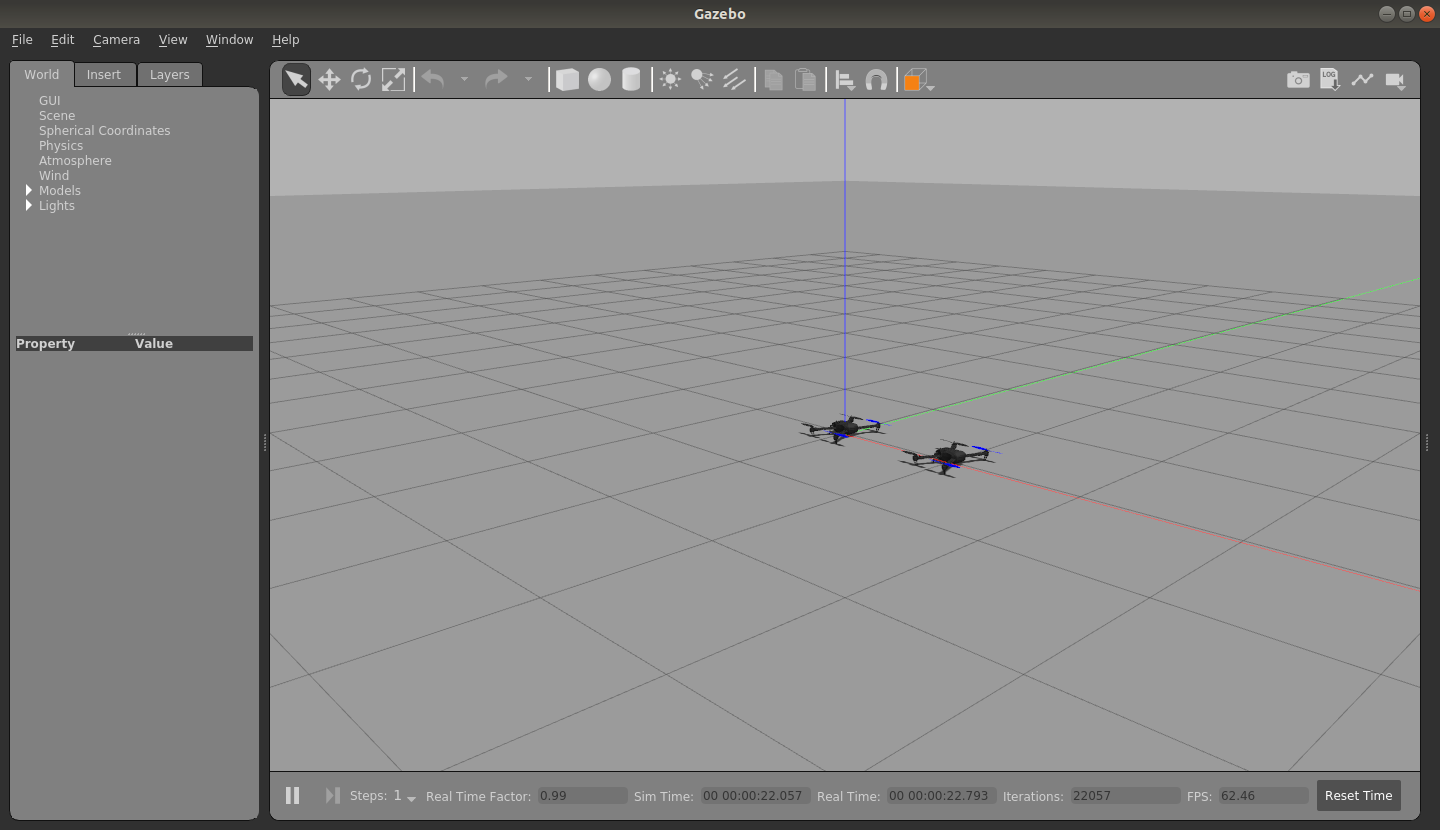
\includegraphics[width=\linewidth]{images/gazebo.png}
  \caption{Gazebo simulation}
\end{figure}